\documentclass[12pt,notitle,letterpaper]{report}
% generated by Docutils <https://docutils.sourceforge.io/>
% rubber: set program xelatex
\usepackage{fontspec}
% \defaultfontfeatures{Scale=MatchLowercase}
% straight double quotes (defined T1 but missing in TU):
\ifdefined \UnicodeEncodingName
  \DeclareTextCommand{\textquotedbl}{\UnicodeEncodingName}{%
    {\addfontfeatures{RawFeature=-tlig,Mapping=}\char34}}%
\fi
\usepackage{ifthen}
\usepackage{alltt}
\usepackage{color}
\usepackage{graphicx}

%%% Custom LaTeX preamble
% Linux Libertine (free, wide coverage, not only for Linux)
\setmainfont{Linux Libertine O}
\setsansfont{Linux Biolinum O}
\setmonofont[HyphenChar=None,Scale=MatchLowercase]{DejaVu Sans Mono}

%%% User specified packages and stylesheets
% embedded stylesheet: c:\git\solar_canopy\rivtManual\solar-canopy-2023\resource\rv00-config\pdf_style.sty
\makeatletter
%%
%% on-c-e default LaTex report class style
%%
\usepackage{lastpage}
\usepackage{fancyhdr}
\usepackage{titlesec}
\usepackage[no-math]{fontspec}
\usepackage{libertine}
\usepackage[libertine]{newtxmath}
\usepackage{currfile}
\usepackage{bm}
\usepackage{gensymb}
\usepackage[normalem]{ulem}
\usepackage{etoolbox}
%% math font
\setmonofont{DejaVu Sans Mono}[Scale=0.8]
\DeclareMathSizes{12}{13}{11}{11}
%% margins
\usepackage{geometry}
\geometry{hmargin={1.0in,0.75in},vmargin={0.9in,1.0in}}
\setlength{\parindent}{0in}

%% pagestyle plain - table of contents
\fancypagestyle{plain} {%
    \fancyhf{}
    \filename@parse{\currfilename}
    \fancyfoot[C]{file: \filename@base .txt \hfill \today\ }
    \renewcommand\headrulewidth{0pt}
    \renewcommand\footrulewidth{1pt}
}

%% pagestyle fancy - calculation
%% header
\pagestyle{fancy}
\fancyhf{}
\fancyhead[L]{\normalsize  Solar Canopy - Larkspur, Ca.}
\fancyhead[R]{\normalsize Page \thepage\ of \pageref*{LastPage} \phantom{aaaaaaaaaa}}
\renewcommand\chaptermark[1]{\markboth{#1}{}}
\renewcommand\sectionmark[1]{\markright{\thesection.\ #1}}
%% footer
\filename@parse{\currfilename}
\fancyfoot[C]{model: \filename@base .txt \hfill \today\ }
\renewcommand\headrulewidth{1pt}
\renewcommand\footrulewidth{1pt}
%% modify section headings - chapters
\titleformat{\chapter}
[display]
{\normalfont\large\bfseries}
{}{0pt}
{\large}
[\vspace{2mm}\titlerule]
\titlespacing*{\chapter}{0pt}{-40pt}{12pt}
%% modify section headings - sections
\titleformat{\section}
[display]
{\normalfont\large\bfseries}
{}{0pt}
{\large}
[\vspace{2mm}\titlerule]
\titlespacing*{\section}{0pt}{-40pt}{12pt}


\makeatother

%%% Fallback definitions for Docutils-specific commands

% class handling for environments (block-level elements)
% \begin{DUclass}{spam} tries \DUCLASSspam and
% \end{DUclass}{spam} tries \endDUCLASSspam
\ifx\DUclass\undefined % poor man's "provideenvironment"
 \newenvironment{DUclass}[1]%
  {% "#1" does not work in end-part of environment.
   \def\DocutilsClassFunctionName{DUCLASS#1}
     \csname \DocutilsClassFunctionName \endcsname}%
  {\csname end\DocutilsClassFunctionName \endcsname}%
\fi

% admonition environment (specially marked topic)
\ifx\DUadmonition\undefined % poor man's "provideenvironment"
 \newbox{\DUadmonitionbox}
 \newenvironment{DUadmonition}%
  {\begin{center}
     \begin{lrbox}{\DUadmonitionbox}
       \begin{minipage}{0.9\linewidth}
  }%
  {    \end{minipage}
     \end{lrbox}
     \fbox{\usebox{\DUadmonitionbox}}
   \end{center}
  }
\fi

% title for topics, admonitions, unsupported section levels, and sidebar
\providecommand*{\DUtitle}[1]{%
  \smallskip\noindent\textbf{#1}\smallskip}
% hyperlinks:
\ifthenelse{\isundefined{\hypersetup}}{
  \usepackage[colorlinks=true,linkcolor=blue,urlcolor=blue]{hyperref}
  \usepackage{bookmark}
  \urlstyle{same} % normal text font (alternatives: tt, rm, sf)
}{}


%%% Body
\renewcommand{\contentsname}{Solar Canopy - Larkspur, Ca.}
\begin{document}
\setcounter{page}{7}

\makeatletter\renewcommand\@dotsep{10000}\makeatother\tableofcontents\listoftables\listoffigures

This report describes the structural design residential solar canopy in
the City of Larkspur, California. It includes the design of a concrete
slab, stem wall, steel tube frame, and attachments of solar panels to the
frame.

The report is divided into the following three divisions:

\begin{itemize}
\item 01 Loads: gravity, wind and seismic

\item 02 Frame: steel tubes, connections and clips

\item 03 Foundation: slab and stem wall
\end{itemize}

Client:

Date:

Location:

The project is located in Larkspur, California.

\noindent\makebox[\linewidth][c]{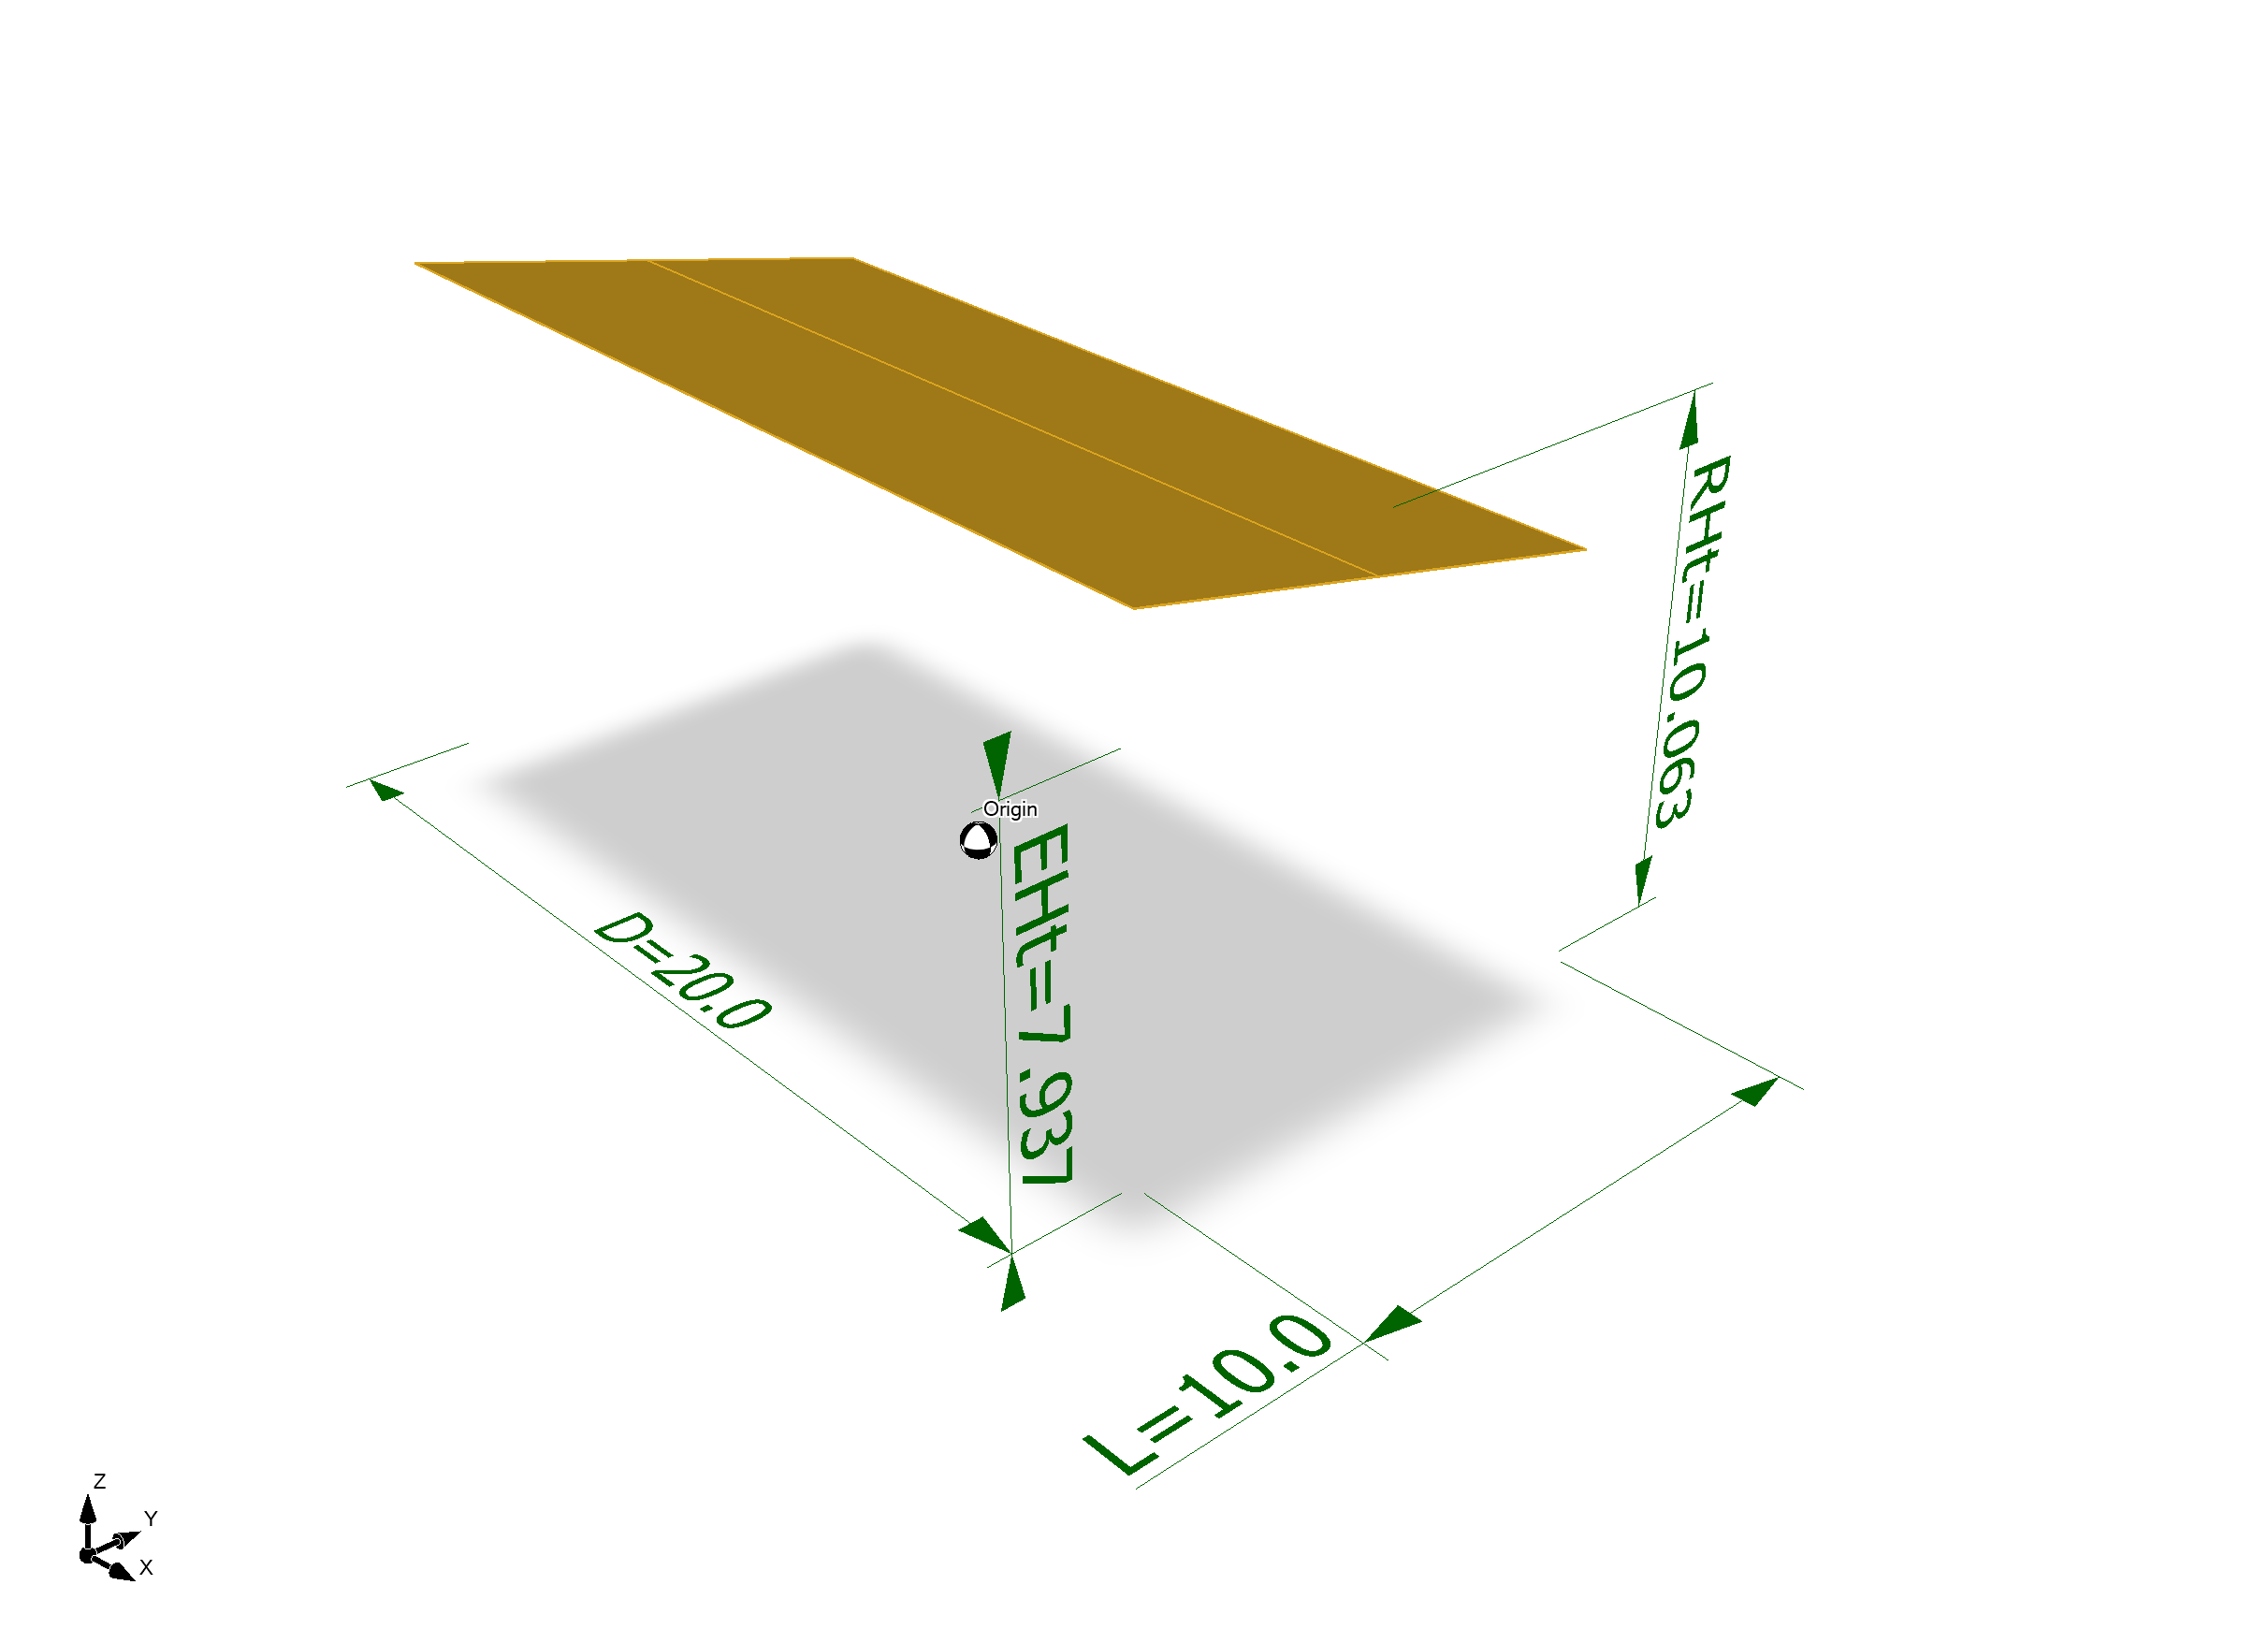
\includegraphics[scale=0.300000]{C:/git/solar_canopy/rivtManual/solar-canopy-2023/resource/rv01-loads/fig1.png}}

\textbf{Wind load 1} \hfill  Fig. 02 {[}02{]}

\noindent\makebox[\linewidth][c]{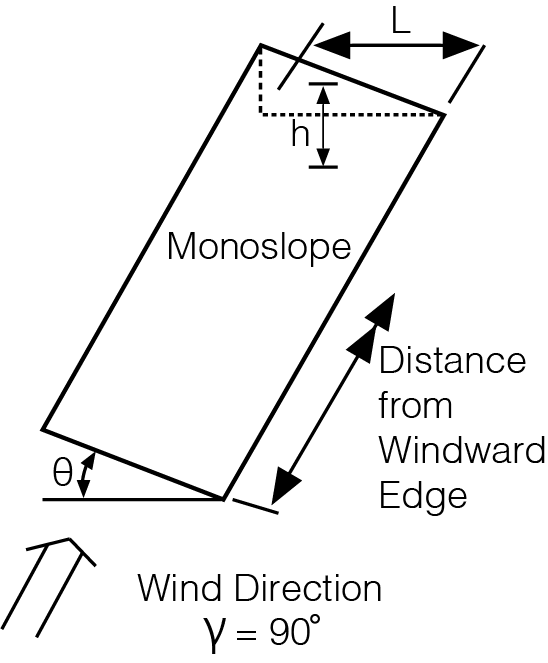
\includegraphics[scale=0.450000]{C:/git/solar_canopy/rivtManual/solar-canopy-2023/resource/rv01-loads/fig2.png}}

\textbf{Wind load 2} \hfill  Fig. 04 {[}02{]}

The permit approval is under the jurisdiction of the City of Larkspur,
California which adopted the 2019 California Building Code {[}CBC{]} and the
2019 California Residential Code {[}CRC{]} as the basis for permiting
requirements of the CBC.

 \begin{tabulary}{1.0\textwidth}{leftleftleft}
%% {llr}
\hline
 Category                                            & Standard   &   Year \\
\hline
 Loading                                             & ASCE-7     &   2016 \\
 Concrete                                            & ACI-318    &   2014 \\
 Wood-National Design Specifications                 & AWC-NDS    &   2018 \\
 Wood-Special Design Provisions for Wind and Seismic & AWC-SDPWS  &   2015 \\
 Wood Frame Construction Manual                      & AWC-WFCM   &   2018 \\
\hline
%% 
\end{tabulary}
\vspace{.15in}

Basic loads and load combinations are derived from the California Building
and Residential Codes.

 \begin{tabulary}{1.0\textwidth}{leftleftleft}
%% {lll}
\hline
 Sym   & Load Effect               & Notes   \\
\hline
 D     & Dead load                 & See IBC 1606 and Chapter 3 of
this publication         \\
 E     & Combined effect of horizontal
and vertical earthquake-
induced forces as defined in
ASCE/SEI 12.4.2                           & See IBC 1613, ASCE/SEI 12.4.2
and Chapter 6 of this
publication         \\
 Em    & Maximum seismic load effect of
horizontal and vertical forces
as set forth in ASCE/SEI
12.4.3                           & See IBC 1613, ASCE/SEI 12.4.3
and Chapter 6 of this
publication         \\
 H     & Load due to lateral earth
pressures, ground water
pressure or pressure of bulk
materials                           & See IBC 1610 for soil lateral
loads         \\
 L     & Live load, except roof live
load, including any permitted
live load reduction                           & See IBC 1607 and Chapter 3 of
this publication         \\
 Li    & Roof live load including any
permitted live load reduction                           & See IBC 1607 and Chapter 3 of
this publication         \\
 R     & Rain load                 & See IBC 1611 and Chapter 3 of
this publication         \\
 W     & Load due to wind pressure & See IBC 1609 and Chapter 5 of
this publication         \\
\hline
%% 
\end{tabulary}
\vspace{.15in}

 \begin{tabulary}{1.0\textwidth}{centercenter}
%% {cc}
\hline
  CBC 2019 reference  &                        Equation                       \\
\hline
    Equation 16-1     &                       1.4(D +F)                       \\
    Equation 16-2     &            1.2(D + F) + l.6(L + H) + 0.5(L            \\
    Equation 16-3     & 1.2(D + F) + l.6(Lr or S or R) + l.6H + (f1L or 0.5W) \\
    Equation 16-4     &   1.2(D + F) + 1.0W + f1L +1.6H + 0.5(Lr or S or R)   \\
    Equation 16-5     &         1.2(D + F) + 1.0E + f1L + l.6H + f2S          \\
    Equation 16-6     &                   0.9D+ l.0W+ l.6H                    \\
    Equation 16-7     &                0.9(D + F) + 1.0E+ l.6H                \\
\hline
%% 
\end{tabulary}
\vspace{.15in}

\newpage

Some filler text

** Table: 02 {[}03{]}** \hfill   Table: 02 {[}03{]}
==========  =======  =========  =================================
variable      value    {[}value{]}  description
==========  =======  =========  =================================
ld1         2.0 psf   0.10 KPa  Urethane foam (4 inch thick)
ld2         1.0 psf   0.05 KPa  Three-ply roofing
ld3         5.0 psf   0.24 KPa  Doug Fir decking 2-in.
ld4         1.0 psf   0.05 KPa  Doug Fir beams 4x12 at 12 ft o.c.
------       ------     ------  ------
roofdl1     9.0 psf   0.43 KPa  Total roof unit load
==========  =======  =========  =================================
** Table: 04 {[}03{]}** \hfill   Table: 04 {[}03{]}
==========  ========  =========  ==========================
variable       value    {[}value{]}  description
==========  ========  =========  ==========================
ld1          3.0 psf   0.14 KPa  3/4 in. hardwood flooring
ld2          2.0 psf   0.10 KPa  1/2 in. plywood subfloor
ld3          4.0 psf   0.19 KPa  2x10 joists at 16 in. o.c.
ld4          1.5 psf   0.07 KPa  fixtures
------        ------     ------  ------
floordl1    10.5 psf   0.50 KPa  Total floor unit load
==========  ========  =========  ==========================
** Table: 06 {[}03{]}** \hfill   Table: 06 {[}03{]}
==========  =======  =========  =============================
variable      value    {[}value{]}  description
==========  =======  =========  =============================
ld1         5.5 psf   0.26 KPa  5/8\textquotedbl{} sheet rock (2)
ld2           2 psf   0.10 KPa  2x4 studs at 16\textquotedbl{} o.c.
ld3         1.5 psf   0.07 KPa  fixtures
------       ------     ------  ------
intwalldl1    9 psf   0.43 KPa  Total interior wall unit load
==========  =======  =========  =============================
** Table: 08 {[}03{]}** \hfill   Table: 08 {[}03{]}
==========  =======  =========  =============================
variable      value    {[}value{]}  description
==========  =======  =========  =============================
ld1         2.0 psf   0.10 KPa  1/2 in plywood sheathing
ld2         2.0 psf   0.10 KPa  2x4 studs at 16 in o.c.
ld3         3.0 psf   0.14 KPa  5/8 in sheet rock
ld4         1.5 psf   0.07 KPa  fixtures
------       ------     ------  ------
extwalldl1  8.5 psf   0.41 KPa  Total exterior wall unit load
==========  =======  =========  =============================
** Table: 10 {[}03{]}** \hfill   Table: 10 {[}03{]}

\textbf{Roof weight} \hfill  Equ. 02 {[}03{]}

\textbf{rfwt1 = arearf1 * roofdl1} \hfill  Equ. 03 {[}03{]}

\textbf{Floor weight} \hfill  Equ. 05 {[}03{]}

\textbf{flrwt1 = areaflr1 * floordl1} \hfill  Equ. 06 {[}03{]}

\textbf{Partition weight} \hfill  Equ. 08 {[}03{]}

\textbf{partwt1 =  htwall1 * lenwall1 * intwalldl1} \hfill  Equ. 09 {[}03{]}

\textbf{Exterior wall weight} \hfill  Equ. 11 {[}03{]}

\textbf{exwallwt1 = htwall1 * lenwall2 * extwalldl1} \hfill  Equ. 12 {[}03{]}

\textbf{Total building weight} \hfill  Equ. 14 {[}03{]}

\textbf{totwt1 = rfwt1 + flrwt1 + partwt1 + exwallwt1} \hfill  Equ. 15 {[}03{]}

** Table: 12 {[}03{]}** \hfill   Table: 12 {[}03{]}

Because the T\&G roof is relatively more flexible, the effective floor load
for seismic models is calculated as the sum of the floor and all of the
partition weight.

\textbf{Effective model floor load} \hfill  Equ. 17 {[}04{]}

\textbf{eflrdl1 = (flrwt1 + partwt1)/(areaflr1)} \hfill  Equ. 18 {[}04{]}

\textbf{Effective model floor density} \hfill  Equ. 20 {[}04{]}

\textbf{eflrdens1 = eflrdl1/(0.5*IN)} \hfill  Equ. 21 {[}04{]}

\textbf{Effective model roof density} \hfill  Equ. 23 {[}04{]}

\textbf{erfdens1 = roofdl1/(1.5*IN)} \hfill  Equ. 24 {[}04{]}

\textbf{Effective model wall density} \hfill  Equ. 26 {[}04{]}

\textbf{ewalldens1 = extwalldl1/(0.5*IN)} \hfill  Equ. 27 {[}04{]}

** Table: 14 {[}04{]}** \hfill   Table: 14 {[}04{]}
.. raw:: latex

\begin{quote}
\newpage
\end{quote}

\begin\{center\} References\end\{center\}

\begin{quote}
\begin{alltt}
ACI
American Concrete Institute
38800 Country Club Drive
Farmington Hills, MI 48331
318—14

AISC
American Institute of Steel
130 East Randolph Street, Suite 2000
Chicago, IL 60601-6219
ANSI/AISC 341—16
Seismic Provisions for Structural Steel Buildings

AISI
American Iron and Steel Institute
25 Massachusetts Avenue, NW Suite 800
Washington, DC 20001
AISI S100—16
North American Specification for the Design of Cold-formed
Steel Structural Members, 2016

ASCE/SEI
American Society of Civil Engineers
Structural Engineering Institute
1801 Alexander Bell Drive
Reston, VA 20191-4400
7—16 Minimum Design Loads and Associated Criteria for
Buildings and Other Structures with Supplement No. 1

AWC
American Wood Council
222 Catoctin Circle SE, Suite 201
Leesburg, VA 20175
ANSI/AWC NDS—2018
National Design Specification (NDS) for
Wood Construction—with 2018 NDS Supplement
ANSI/AWC SDPWS—2015
Special Design Provisions for Wind and Seismic

CBC
International Code Council
500 New Jersey Avenue, NW
6th Floor, Washington, DC 20001
California Building Standards Commission
2525 Natomas Park Dr # 130, Sacramento, CA 95833
California Building Code
Part 2 of Title 24, 2019 Edition

CRC
International Code Council
500 New Jersey Avenue, NW
6th Floor, Washington, DC 20001
California Building Standards Commission
2525 Natomas Park Dr # 130, Sacramento, CA 95833
California Residential Code
Part 2.5 of Title 24, 2019 Edition
\end{alltt}
\end{quote}

\newpage

\begin\{center\} Drawings\end\{center\}

\begin{quote}
\begin{alltt}
55 LORING - RESIDENCE REMODEL AND SEISMIC STRENGTHENING

PR.01: COVER AND INDEX
PR.02: PROJECT SCOPE
PR.03: GENERAL NOTES, CONTRACTORS
PR.04: SITE PLAN
PR.05: PLANS
PR.06: ELEVATIONS
PR.07: KITCHEN AND BATH REMODEL
PR.08: MASTER BATH, CLOSET, LAUNDRY
PR.09: RESIDENCE STRENGTHENING
PR.10: CARPORT STRENGTHENING
PR.11: SITE IMPROVEMENTS
\end{alltt}
\end{quote}

\newpage

\begin\{center\} Abbreviations - Terms\end\{center\}
.. raw:: latex

\begin{quote}
begin\{center\}textbf\{Text\}end\{center\}
setlength\{parindent\}\{0.2in\}
hspace*\{4cm\} = kill
begin\{tabbing\}

\begin{DUclass}{system-message}
\begin{DUadmonition}
\DUtitle{system-message
}

{\color{red}ERROR/3} in \texttt{c:\textbackslash{}git\textbackslash{}solar\_canopy\textbackslash{}rivtManual\textbackslash{}solar-canopy-2023\textbackslash{}resource\textbackslash{}rv00-config\textbackslash{}temp\textbackslash{}r0101.rst}, line~332

Unexpected indentation.
backrefs: \end{DUadmonition}
\end{DUclass}

\begin{quote}
indenttextbf\{\}         >  \{\}\textbackslash{}
indenttextbf\{ASD\}      >  \{Allowable Stress Design\}\textbackslash{}
indenttextbf\{ACI\}      >  \{American Concrete Institute\}\textbackslash{}
indenttextbf\{AISC\}     >  \{American Institute of Steel Construction\}\textbackslash{}
indenttextbf\{AISI\}     >  \{American Iron and Steel Institute\}\textbackslash{}
indenttextbf\{ASTM\}     >  \{American Society for Testing and Materials\}\textbackslash{}
indenttextbf\{AWS\}      >  \{American Welding Society\}\textbackslash{}
indenttextbf\{AB\}       >  \{Anchor Bolt\}\textbackslash{}
indenttextbf\{BDRY\}     >  \{Boundry\}\textbackslash{}
indenttextbf\{CBC\}      >  \{Califiornia Building Code\}\textbackslash{}
indenttextbf\{CRC\}      >  \{Califiornia Residential Code\}\textbackslash{}
indenttextbf\{CIP\}      >  \{Cast-In-Place\}\textbackslash{}
indenttextbf\{CLR\}      >  \{Clear\}\textbackslash{}
indenttextbf\{CONC\}     >  \{Concrete\}\textbackslash{}
indenttextbf\{CMU\}      >  \{Concrete Masonry Unit\}\textbackslash{}
indenttextbf\{CRSI\}     >  \{Concrete Reinforcing Steel Institute\}\textbackslash{}
indenttextbf\{CONST JT\} >  \{Construction Joint\}\textbackslash{}
indenttextbf\{CONT\}     >  \{Continuous\}\textbackslash{}
indenttextbf\{CJ\}       >  \{Control Joint\}\textbackslash{}
indenttextbf\{D-C\}      >  \{Demand-Capacity (ratio)\}\textbackslash{}
indenttextbf\{DIA\}      >  \{Diameter\}\textbackslash{}
indenttextbf\{DIM\}      >  \{Dimension\}\textbackslash{}
indenttextbf\{EA\}       >  \{Each\}\textbackslash{}
indenttextbf\{EF\}       >  \{Each Face\}\textbackslash{}
indenttextbf\{EJ\}       >  \{Expansion Joint\}\textbackslash{}
indenttextbf\{ES\}       >  \{Each Side\}\textbackslash{}
indenttextbf\{EW\}       >  \{Each Way\}\textbackslash{}
indenttextbf\{EXP Bolt\} >  \{Expansion Bolt\}\textbackslash{}
indenttextbf\{EXP JT\}   >  \{Expansion Joint\}\textbackslash{}
indenttextbf\{FTG\}      >  \{Footing\}\textbackslash{}
indenttextbf\{FND\}      >  \{Foundation\}\textbackslash{}
indenttextbf\{GALV\}     >  \{Galvanized\}\textbackslash{}
indenttextbf\{GA\}       >  \{Gauge\}\textbackslash{}
indenttextbf\{GR\}       >  \{Grade\}\textbackslash{}
indenttextbf\{HT\}       >  \{Height\}\textbackslash{}
indenttextbf\{IN\}       >  \{Inch\}\textbackslash{}
indenttextbf\{ID\}       >  \{Inside Diameter\}\textbackslash{}
indenttextbf\{ICBO\}     >  \{International Conference of Building Officials\}\textbackslash{}
indenttextbf\{K\}        >  \{Kip (1000 Pounds)\}\textbackslash{}
indenttextbf\{LWC\}      >  \{Light Weight Concrete\}\textbackslash{}
indenttextbf\{LRFD\}     >  \{Load and Resistance Factor Design\}\textbackslash{}
indenttextbf\{NWC\}      >  \{Normal Weight Concrete\}\textbackslash{}
indenttextbf\{NIC\}      >  \{Not in Contract\}\textbackslash{}
indenttextbf\{OC\}       >  \{On Center\}\textbackslash{}
indenttextbf\{OD\}       >  \{Outside Diameter\}\textbackslash{}
indenttextbf\{OPNG\}     >  \{Opening\}\textbackslash{}
indenttextbf\{PVC\}      >  \{Polyvinyl Chloride\}\textbackslash{}
indenttextbf\{PSF\}      >  \{Pounds per Square Foot\}\textbackslash{}
indenttextbf\{PSI\}      >  \{Pounds per Square Inch\}\textbackslash{}
indenttextbf\{R\}        >  \{Radius\}\textbackslash{}
indenttextbf\{REINF\}    >  \{Reinforced\}\textbackslash{}
indenttextbf\{SIM\}      >  \{Similar\}\textbackslash{}
indenttextbf\{SOG\}      >  \{Slab on Grade\}\textbackslash{}
indenttextbf\{SL\}       >  \{Splice Length\}\textbackslash{}
indenttextbf\{SQ\}       >  \{Square\}\textbackslash{}
indenttextbf\{STD\}      >  \{Standard\}\textbackslash{}
indenttextbf\{SDI\}      >  \{Steel Deck Institute\}\textbackslash{}
indenttextbf\{SF\}       >  \{Step Footing or Square Foot\}\textbackslash{}
indenttextbf\{SYM\}      >  \{Symmetrical\}\textbackslash{}
indenttextbf\{THK\}      >  \{Thick or Thickness\}\textbackslash{}
indenttextbf\{T \& B\}   >  \{Top and Bottom\}\textbackslash{}
indenttextbf\{T \& G\}   >  \{Tongue and Groove\}\textbackslash{}
indenttextbf\{TOC\}      >  \{Top of Concrete\}\textbackslash{}
indenttextbf\{TOF\}      >  \{Top of Foundation\}\textbackslash{}
indenttextbf\{TOS\}      >  \{Top of Steel\}\textbackslash{}
indenttextbf\{TOW\}      >  \{Top of Wall\}\textbackslash{}
indenttextbf\{TYP\}      >  \{Typical\}\textbackslash{}
indenttextbf\{UNO\}      >  \{Unless Noted Otherwise\}\textbackslash{}
indenttextbf\{WWF\}      >  \{Welded Wire Fabric\}\textbackslash{}
indenttextbf\{W/\}       >  \{With\}\textbackslash{}
indenttextbf\{WP\}       >  \{Working Point\}\textbackslash{}
\end{quote}

\begin{DUclass}{system-message}
\begin{DUadmonition}
\DUtitle{system-message
}

{\color{red}WARNING/2} in \texttt{c:\textbackslash{}git\textbackslash{}solar\_canopy\textbackslash{}rivtManual\textbackslash{}solar-canopy-2023\textbackslash{}resource\textbackslash{}rv00-config\textbackslash{}temp\textbackslash{}r0101.rst}, line~403

Block quote ends without a blank line; unexpected unindent.
backrefs: \end{DUadmonition}
\end{DUclass}

end\{tabbing\}
\end{quote}

\newpage

\begin\{center\} Abbreviations - Math\end\{center\}
.. raw:: latex

\begin{quote}
\begin{description}
\item[{begin\{align\}}] 
bm\{D\}       \& = textrm\{dead load\}                               \textbackslash{}
bm\{L\}       \& = textrm\{live load\}                               \textbackslash{}
bm\{D\_m\}     \& = textrm\{module dead load\}                        \textbackslash{}
bm\{E\}       \& = textrm\{earthquake load\}                         \textbackslash{}
bm\{F\_a\}     \& = textrm\{acceleration site coefficient\}           \textbackslash{}
bm\{F\_v\}     \& = textrm\{velocity site coefficient\}               \textbackslash{}
bm\{F\_N\}     \& = textrm\{normal wind force\}                       \textbackslash{}
bm\{GC\_M\_s\}  \& = textrm\{net moment static coefficient\}           \textbackslash{}
bm\{GC\_M\_d\}  \& = textrm\{net moment dynamic coefficient\}          \textbackslash{}
bm\{GC\_M\}    \& = textrm\{net moment coefficient\}                  \textbackslash{}
bm\{GC\_P\}    \& = textrm\{net pressure coefficient\}                \textbackslash{}
bm\{GC\_P\_s\}  \& = textrm\{net static pressure coefficient\}         \textbackslash{}
bm\{GC\_P\_d\}  \& = textrm\{net dynamic pressure coefficient\}        \textbackslash{}
bm\{k\_1\}     \& = textrm\{hazard coefficient\}                      \textbackslash{}
bm\{k\_2\}     \& = textrm\{terrain and structure coefficient\}       \textbackslash{}
bm\{k\_3\}     \& = textrm\{topography coefficient\}                  \textbackslash{}
bm\{Kzt\}     \& = textrm\{topographic Factor\}                      \textbackslash{}
bm\{K\_z\}     \& = textrm\{velocity pressure exposure coefficient\}  \textbackslash{}
bm\{MRI\}     \& = textrm\{mean return interval\}                    \textbackslash{}
bm\{p\_d\}     \& = textrm\{net design wind pressure on module - Pa\} \textbackslash{}
bm\{SDOF\}    \& = textrm\{single degree of freedom\}                \textbackslash{}
bm\{S\_s\}     \& = textrm\{short period mapped acceleration\}        \textbackslash{}
bm\{S\_D\_S\}   \& = textrm\{site design response acceleration\}       \textbackslash{}
bm\{S\_1\}     \& = textrm\{1 second period mapped acceleration\}     \textbackslash{}
bm\{S\_M\_S\}   \& = textrm\{short period parameter\}                  \textbackslash{}
bm\{S\_M\_1\}   \& = textrm\{1 second period parameter\}               \textbackslash{}
bm\{T\}       \& = textrm\{fundamental period of structure\}         \textbackslash{}
bm\{M\_t\_o\_r\} \& = textrm\{wind moment about panel center \}         \textbackslash{}
bm\{T\_0\}     \& = textrm\{short period spectral cap \}              \textbackslash{}
bm\{T\_S\}     \& = textrm\{long period spectral cap\}                \textbackslash{}
bm\{V\_b\}     \& = textrm\{basic wind speed\}                        \textbackslash{}
bm\{V\_B\}     \& = textrm\{seismic design base shear\}               \textbackslash{}
bm\{W\}       \& = textrm\{wind load\}                               \textbackslash{}
bm\{W\}       \& = textrm\{seismic weight of structure \}            \textbackslash{}

\end{description}

\begin{DUclass}{system-message}
\begin{DUadmonition}
\DUtitle{system-message
}

{\color{red}WARNING/2} in \texttt{c:\textbackslash{}git\textbackslash{}solar\_canopy\textbackslash{}rivtManual\textbackslash{}solar-canopy-2023\textbackslash{}resource\textbackslash{}rv00-config\textbackslash{}temp\textbackslash{}r0101.rst}, line~450

Definition list ends without a blank line; unexpected unindent.
backrefs: \end{DUadmonition}
\end{DUclass}

end\{align\}
\end{quote}

\end{document}
